\documentclass{blue-book}
\NoteNumber{1}

\usepackage{graphicx}

\usepackage{amsmath}

\newcommand{\gwendolen}{{\sc Gwendolen}}

\newcommand{\INThddeed}{\ensuremath{\mathit{\AILhd_d}}}
\newcommand{\INThdunifier}[1]{\ensuremath{\AILunifier^{\AILhd(#1)}}}
\newcommand{\INTtl}{\ensuremath{\AILtl_i}}
\newcommand{\INTcons}{\ensuremath{\AILcons_p}}
\newcommand{\INTmergeunifier}{\ensuremath{{\tt U}_{\AILunifier}}}
\newcommand{\INThdevent}{\ensuremath{\AILhd_e}}
\newcommand{\INTnew}{\ensuremath{{\tt new}}}

\newcommand{\AILagent}{\ensuremath{\mathit{ag}}}
\newcommand{\AILbelief}{\ensuremath{\mathit{b}}}
\newcommand{\AILbeliefbase}{\ensuremath{\mathit{B}}}
\newcommand{\AILunifier}{\ensuremath{\theta}}
\newcommand{\AILhd}{\ensuremath{{\tt hd}}}
\newcommand{\AILcons}{\ensuremath{{\tt ;}}}
\newcommand{\AILtl}{\ensuremath{{\tt tl}}}
\newcommand{\AILintention}{\ensuremath{\mathit{i}}}
\newcommand{\AILaction}{\ensuremath{\mathit{a}}}
\newcommand{\AILgoal}{\ensuremath{\mathit{g}}}
\newcommand{\AILgoaltype}{\ensuremath{\mathit{\tau_{\AILgoal}}}}
\newcommand{\AILdo}{\ensuremath{\mathrm{\mathbf{do}}}}
\newcommand{\AILmessage}{\ensuremath{\mathit{m}}}
\newcommand{\AILnpy}{\ensuremath{\epsilon}}
\newcommand{\AILprobgoal}[2]{\ensuremath{\mathit{\mathtt{x}!_{#1}#2}}}
\newcommand{\AILwaitfor}[1]{\ensuremath{*\ldots{#1}}}
\newcommand{\AILsuspended}{\bf is\_suspended}
\newcommand{\AILintset}{\ensuremath{\mathit{I}}}
\newcommand{\AILsuspend}{{\tt suspend}}
\newcommand{\AILunsuspend}{\bf unsuspend}
\newcommand{\AILadd}[1]{\ensuremath{\mathit{+#1}}}
\newcommand{\AILevent}{\ensuremath{\mathit{e}}}
\newcommand{\AILdeed}{\ensuremath{\mathit{d}}}

\newcommand{\sentmessage}[2]{\ensuremath{\mathit{\uparrow^{#1}#2}}}

\newcommand{\inlinecode}[1]{\mbox{\texttt{#1}}}

\newenvironment{stacksed}{
\begin{tabular}{l|l} 
\hline
event & deed  \\ 
\hline \hline} {
\cr \hline 
\end{tabular}
}


\title{Action Lifecycles in \gwendolen}

\begin{document}
\maketitle

Way back in the before times when it was possible to meet in person, Peter, Rafael and I sat down and brainstormed what the \gwendolen\ semantics might look like if it explicitly recognised that actions might take time to complete and that they could complete with success, failure or timeout (as discussed more generally in~\cite{dennis14,dennis14:_action_durat_failur_bdi_languag}).  The result was a set of scrawled diagrams and greek letters that now, 10 months later, even I have trouble interpreting.  So this is a second attempt at producing something intelligable.

\section{Intentions in \gwendolen}
\label{sec:intentions}

Intentions are crucial to understanding \gwendolen.  BDI languages use intentions to
store the \emph{intended means} for achieving goals -- this is
generally represented as some from of {\em deed stack} (deeds include
actions, belief updates, and the commitment to
goals)\index{deed!stack}.  Intention structures 
also maintain information about the (sub-)goal they are intended to
achieve or the event that triggered them. \gwendolen\ aggregates
this information: an intention becomes a stack of tuples of an
event\index{event}, a deed\index{deed}, and a
unifier\index{unifier} (but I'm going to ignore unifiers in everything that follows as an added complexity which we can deal with later).  This tuple is most
simply viewed as a matrix structure consisting of two columns in
which we record events (new perceptions, goals committed to and so
forth),  and deeds (a plan of future actions, belief updates, goal
commitments, etc.). These columns form an event stack and a deed
stack.  Rows associate a
particular deed with the event that has caused the deed to be placed
on the intention. New events are associated with an empty
deed, $\AILnpy$.

\paragraph{Example} The following shows the structure for a
single intention to clean a room.  We use a standard BDI syntax: $!g$
to indicate the goal $g$, and $+!g$ to indicate the commitment to
achieve that goal (i.e., a new goal that $g$ becomes true is
adopted)\index{goal!commitment}. 
\begin{center}
        \begin{stacksed}
                \inlinecode{+!clean()} & \inlinecode{+!goto(room1)} \\
                \inlinecode{+!clean()} & \inlinecode{+!vacuum(room1)}  
        \end{stacksed}
\end{center}
This intention has been triggered by a goal to clean --- the
commitment to the goal
$clean()$ is the trigger event for both rows in the intention.  An
intention is processed from top to bottom so we see here that the
agent first intends to commit to the goal $goto(room1)$.   Once it has committed
to that goal it then commits to the goal $\mathit{vacuum}(room1)$.  In \gwendolen\ the process of committing to a goal causes an expansion of
the intention stack, first making the goal into an event which has yet to be planned (so is associated with the empty deed $\AILnpy$) and then selecting a plan to execute which replaces $\AILnpy$ and pushes more deeds on the intention to be processed.  


If 
$goto(room1)$ is an achievement goal (which among other things means it it remains on the deed stack until it is ``achieved'') then our intention is expanded
\emph{before} the agent commits to vacuuming the room and
the above intention becomes first
\begin{center}
        \begin{stacksed}
                \inlinecode{+!goto(room1)} & \AILnpy \\
                 \inlinecode{+!clean()} & \inlinecode{+!goto(room1)} \\
               \inlinecode{+!clean()} & \inlinecode{+!vacuum(room1)} 
        \end{stacksed}
\end{center}
and maybe then (depending upon the plan)
\begin{center}
        \begin{stacksed}
                \inlinecode{+!goto(room1)} &
\inlinecode{+!planRoute(room1)}  \\
                \inlinecode{+!goto(room1)} &
\inlinecode{+!follow\_route} \\
                \inlinecode{+!goto(room1)} & \inlinecode{+!enter(room1)} \\
                  \inlinecode{+!clean()} & \inlinecode{+!goto(room1)} \\
               \inlinecode{+!clean()} & \inlinecode{+!vacuum(room1)} 
        \end{stacksed}
\end{center}

At any moment, we assume there is a \emph{current intention}\index{intention!in gwendolen} which is
the one being processed at that time. 
The stacks that form the intention are further paired with two booleans, \emph{suspended}, and \emph{locked}
which indicate the intention's status.
A suspended intention is, by default, \emph{not}
selected at the intention selection phase of the agent's reasoning.  

Because intentions are stacks we are often interested the top row of the intention, \emph{the head}, written $\AILhd_{\AILintention}(\AILintention)$, and the rest of the intention, \emph{the tail}, written $\INTtl(\AILintention)$.  Sometimes we are just interested in the top event on the intention, $\INThdevent$ or the top deed on the intention, $\INThddeed$.

\section{How actions Currently work in \gwendolen}
Currently actions with durations work via a kludge in \gwendolen, in which the action is started using an action command on the top of an intention's deed stack and then the intention is suspended until some success condition for the action is  reached using a ``wait for'' command.  In most BDI languages an action starts and the agent stops doing anything else until the action completes, but this doesn't really work for lots of the systems we consider.  In particular when an action involves moving from one location to another we generally want to continue monitoring for other things (like approaching collisions, thruster failures, etc.) while the robot is moving and this can't happen if all processing within the agent is basically locked until the action finishes.

In the \gwendolen\ semantics this is represented by Equation~\eqref{eq:action} (which I've simplified a bit from the rule in the published semantics by removing all reference to unifiers, edge cases like the action command throwing an error, and checks that isn't a \emph{send message} action which has a special rule).  The notation I'm using has conditions for a transition above the line, and the actual transition below the line.  In this case I'm representing the state of the system as the pair of an environment, $\xi$, and a big tuple representing all the parts of the agent such as its belief base, goal base, current intention, other intentions, plans, reasoning rules, message inbox etc.. etc., (lots of detail that I'm going to gloss over here).

\begin{equation}
  \frac{
    \INThddeed(\AILintention) = \AILaction
\quad \xi \xrightarrow{\AILdo(\AILaction)} \xi' 
}{
\langle \xi, \langle \ldots \AILintention \ldots \rangle \rangle \rightarrow_{\tt action} 
\langle \xi', \langle \ldots \INTtl(\AILintention)  \ldots \rangle \rangle
}
\label{eq:action}
\end{equation}

So if the top deed on the intention is an action, $\INThddeed(\AILintention) = \AILaction$, and the change the action makes to the environment, $\xi$, is to turn it into $\xi'$, represented by $ \xi \xrightarrow{\AILdo(\AILaction)} \xi' $ then performing the action transforms the pair of the environment and agent by transforming the environment and removing the top row from the current intention, $\AILintention$, ($\AILintention$ becomes $\INTtl(\AILintention)$).  All other parts of the agent state are unchanged (represented by the liberal use of $\ldots$).

Meanwhile the rules for handling wait for are:

\begin{equation}
\frac{\begin{array}{c}
\INThddeed(\AILintention) = \AILwaitfor{\AILbelief}
\quad B, R \models \AILbelief
\end{array}
}{
\begin{array}{c}
  \langle \xi, \langle \ldots \AILintention \ldots \AILbeliefbase, R \ldots \rangle \rangle
\rightarrow_{\tt wait\_for} 
\langle \xi, \langle \ldots
\INTtl(\AILintention)
\ldots \AILbeliefbase, R \ldots \rangle ) \rangle
\end{array}
}
\label{eq:waitfor1}
\end{equation}

\begin{equation}
\frac{
\begin{array}{c}
  \INThddeed(\AILintention) = \AILwaitfor{\AILbelief}
\quad B, R \not \models \AILbelief
\end{array}
}{
\begin{array}{c}
  \langle \xi, \langle \ldots \AILintention, \ldots, \AILbeliefbase, R \ldots \rangle \rangle
\rightarrow_{\tt wait\_for} 
\langle \xi', \langle \ldots
\AILsuspend(\AILintention),
\ldots, \AILbeliefbase, R \ldots
\rangle  \rangle
\label{eq:waitfor2}
\end{array}
}
\end{equation}
where $B, R \models b,$ means that the
formula $b$ follows using Prolog-style reasoning from the agent's belief base and Prolog rule-base.  $\AILsuspend(\AILintention)$ suspends an intention. 

So, if an intention is waiting for some belief, $\AILbelief$, to become true ($\AILwaitfor{\AILbelief}$) then if that belief is alreadly/now true the intention continues processing \eqref{eq:waitfor1}.  Otherwise
the intention is suspended \eqref{eq:waitfor2}.   There's a special case for when there are no unsuspended intentions, but I'm ignoring that for now.

Lastly, intentions get unsuspended when new beliefs are added:
\begin{equation}
\frac{\INThddeed(\AILintention)  = +\AILbelief
}{
\begin{array}{c}
\langle \xi, \langle \ldots \AILintention, \AILintset, \AILbeliefbase \ldots \rangle \rangle \rightarrow_{\tt add\_belief} \\
\langle \xi, \langle \ldots
\INTtl(\AILintention) , 
\AILunsuspend(\AILintset, \AILbelief) \cup \INTnew(\AILadd \AILbelief, \AILnpy), 
\AILbeliefbase \cup \{\AILbelief\}, \ldots \rangle \rangle
\end{array}
}
\end{equation}
where $\AILunsuspend(\AILintset, \AILbelief)$ unsuspends all suspended intentions in $\AILintset$ that are waiting for $\AILbelief$ to become true (this is actually concealing a multitude of sins since sometimes reasoning rules are needed to determine if an intention should be unsuspended).  $\INTnew(\AILevent, \AILdeed)$ creates a new intention from an event and a deed. 

This rule adds new belief to the belief base and a new intention noting the appearance of the new belief.  At the same time it unsuspends all intentions which are waiting for $b$ to be achieved as part of their suspend condition.

\section{New Proposal}

\newcommand{\newaction}[4]{\ensuremath{#1:(#2,#3,#4)}}

The new proposal is that actions should be paired with a success, failure and abort condition.  I'm going to write this as $\newaction{\AILaction}{\phi_s}{\phi_f}{\phi_a}$ where $\phi_s$ is the success condition, $\phi_f$ is the failure condition and $\phi_a$ is the abort condition.  And we obviously want some semantics that looks a bit like a mash up of our action and wait for transition rules -- except in the case of failure/abort we don't want to just carry on processing the intention, we want to do something else!!

This is where the diagram about goal life cycles came in which we adapted (I think,  looking at our scrawl) to be something like:

\begin{center}
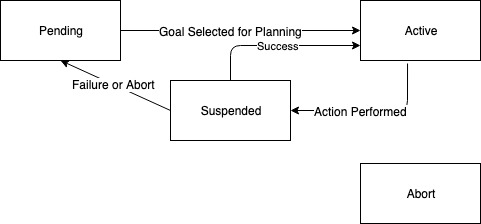
\includegraphics[width=3in]{images/lifecycle.jpg}
\end{center}

A goal that is \emph{Pending} is a goal on the top of an intention paired with a ``no plan yet'' deed ($\AILnpy$) which we discussed in Section~\ref{sec:intentions}.  When the intention is selected and a plan is applied to the goal, expanding the intention, it becomes \emph{Active}.  When the top deed is an action then the whole intention is suspended, and this is what we mean by the Goal being \emph{Suspended} in the lifecycle.  If the action completes with sucess then the intention becomes active again and continues processing (like in the existing Wait For case).  \emph{However} if the goal fails or aborts then we drop everything to do with the current plan and go back to the pending state.  We don't really distinguish between failures and aborts -- the distinction might be useful for diagnosis, but doesn't make much difference to goal processing.

There is also an \emph{Abort} state where we might want to abandon the goal entirely, not just attempt to replan it -- there is a drop goal method in the AIL which should do this.  Judging by our scribbles we weren't certain when a goal should be aborted altogether but it might be after repeated planning failures.

So if I were to make a first pass at adapted rules, I would change the action rule to something like: 

\begin{equation}
  \frac{
    \INThddeed(\AILintention) = \newaction{\AILaction}{\phi_s}{\phi_f}{\phi_a}
\quad \xi \xrightarrow{\AILdo(\AILaction)} \xi'  \quad B, R \models \phi_s
}{
\langle \xi, \langle \ldots \AILintention, B, R, \ldots \rangle \rangle \rightarrow_{\tt action} 
\langle \xi', \langle \ldots \INTtl(\AILintention), B, R \ldots \rangle \rangle
}
\label{eq:action_success}
\end{equation}

\begin{equation}
  \frac{
    \INThddeed(\AILintention) = \newaction{\AILaction}{\phi_s}{\phi_f}{\phi_a}
\quad \xi \xrightarrow{\AILdo(\AILaction)} \xi'  \quad B, R \models \phi_f \lor B, R \models \phi_a
}{
\langle \xi, \langle \ldots \AILintention, B, R, \ldots \rangle \rangle \rightarrow_{\tt action} 
\langle \xi', \langle \text{whatever happens when we go back to pending} \rangle \rangle
}
\label{eq:action_fail}
\end{equation}

\begin{equation}
  \frac{
    \INThddeed(\AILintention) = \newaction{\AILaction}{\phi_s}{\phi_f}{\phi_a}
\quad \xi \xrightarrow{\AILdo(\AILaction)} \xi'  \quad B, R \not \models \phi_s \quad B, R \not \models \phi_f \quad B, R \not \models \phi_a
}{
\langle \xi, \langle \ldots \AILintention, B, R, \ldots \rangle \rangle \rightarrow_{\tt action} 
\langle \xi', \langle \ldots \AILsuspend(\mathbf{done}(\AILintention)), B, R \ldots \rangle \rangle
}
\label{eq:action_new}
\end{equation}

So if the action succeeds immediately (or trivially) \eqref{eq:action_success} then we carry on processing the intention in an \emph{Active} state.  If the action fails immediately \eqref{eq:action_fail} we do ``whatever'' (I could probably write this out, but it would require some thought and probably more notation and isn't needed just at this point) and if the action neither succeeds nor fails immediately then we suspend the intention with some marker, $\mathbf{done}$ to show we've actually performed the action.

When we unsuspend intentions when we add beliefs we can extend $\AILunsuspend$ further to check these ``done"\footnote{To be honest I'm not sure a $\mathbf{done}$ annotation is the best way to do this, but I think it suffices for now and we can see how the implementation works out first.} actions.

And then we have:

\begin{equation}
  \frac{
    \INThddeed(\AILintention) = \mathbf{done}(\newaction{\AILaction}{\phi_s}{\phi_f}{\phi_a})  \quad B, R \models \phi_s
}{
\langle \xi, \langle \ldots \AILintention, B, R, \ldots \rangle \rangle \rightarrow_{\tt action} 
\langle \xi', \langle \ldots \INTtl(\AILintention), B, R \ldots \rangle \rangle
}
\label{eq:done_action_success}
\end{equation}

\begin{equation}
  \frac{
    \INThddeed(\AILintention) = \mathbf{done}(\newaction{\AILaction}{\phi_s}{\phi_f}{\phi_a})
\quad B, R \models \phi_f \lor B, R \models \phi_a
}{
\langle \xi, \langle \ldots \AILintention, B, R, \ldots \rangle \rangle \rightarrow_{\tt action} 
\langle \xi', \langle \text{whatever happens when we go back to pending} \rangle \rangle
}
\label{eq:done_action_fail}
\end{equation}

\begin{equation}
  \frac{
    \INThddeed(\AILintention) = \mathbf{done}(\newaction{\AILaction}{\phi_s}{\phi_f}{\phi_a})
\quad B, R \not \models \phi_s \quad B, R \not \models \phi_f \quad B, R \not \models \phi_a
}{
\langle \xi, \langle \ldots \AILintention, B, R, \ldots \rangle \rangle \rightarrow_{\tt action} 
\langle \xi', \langle \ldots \AILsuspend(\mathbf{done}(\AILintention)), B, R \ldots \rangle \rangle
}
\label{eq:done_action_new}
\end{equation}

Which are the same as the new action rules except they don't actually try to do the action,  they just check if the action has finished yet.  To be honest we shouldn't need \eqref{eq:done_action_new} since the intention should only become unsuspended if one of the three conditions is true, but I'm including it just in case there is some weird scenario I've not thought of where it is needed.

\bibliography{bluebook}
\bibliographystyle{apalike}

\end{document}